\documentclass[10pt]{beamer}
\usetheme{Berlin}
\usecolortheme{lily}
\usepackage[utf8x]{inputenc}
\usepackage[english]{babel}
\usepackage[T1]{fontenc}
\usepackage{lmodern}
\usepackage{amsmath}
\usepackage{amssymb}
\usepackage{enumerate}
\usepackage{graphicx}
\usepackage{cite}
\usepackage{listings}
\usepackage{hyperref}
\usepackage{lipsum}
\usepackage{tikz}
\beamertemplatenavigationsymbolsempty

%\usepackage{pgfpages}
%\setbeameroption{show notes}
%\setbeameroption{show notes on second screen=left}

\newcommand{\docauthor}{Axel Angel}
\newcommand{\doctitle}{Towards Distortion-Predictable Embedding of Neural Networks}
\newcommand{\docsubtitle}{Presentation}
\newcommand{\eg}{e.g.}
\newcommand{\reff}[1]{~\ref{#1}}
\setkeys{Gin}{width=1.0\textwidth}

\author{\docauthor}
\title{\doctitle}

\pdfinfo{
    /Author (\docauthor)
    /Title (\doctitle)
    /Subject (\docsubtitle)
    }

\begin{document}
\begin{frame}
    \titlepage
    \begin{center}
        Supervised by: Pascal Fua.
        \\
        \vspace{0.5cm}
        \includegraphics[width=3cm]{../report/thesis_figures/epfl_logo.png}
    \end{center}
\end{frame}

% more why = explain why
% explain recap orally the goal: 1-2 sentences
% study of properties of CNN, embedding,
% predictable = control over embedding
% (before title)

\begin{frame}
    \tableofcontents{}
\end{frame}

\section{Motivations}
\begin{frame}
    \frametitle{Motivations}
    \begin{itemize}
        \item Face recognition
        \item Develop the theory behind it
        \item Our work is a start
    \end{itemize}

    \begin{figure}[h]
        \begin{center}
            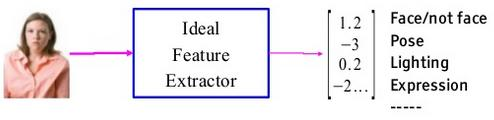
\includegraphics[width=0.75\textwidth]{figures/lecun_face_reco.jpg}
        \end{center}
    \end{figure}
    % fixme: add figure (LeCun, face reco)
    % what we want to do with face reco, not really clear
    % feed person picture into network, now abstract features, but want something more controllable, predictable (pose, expression, identity : separately)
\end{frame}

\section{Review of CNNs}
\begin{frame}
    \frametitle{Review of CNNs}
    \begin{itemize}
        \item Architecture
        \item Similar to a blackbox
        \item We focus on the embedding
    \end{itemize}

    \begin{figure}[h]
        \begin{center}
            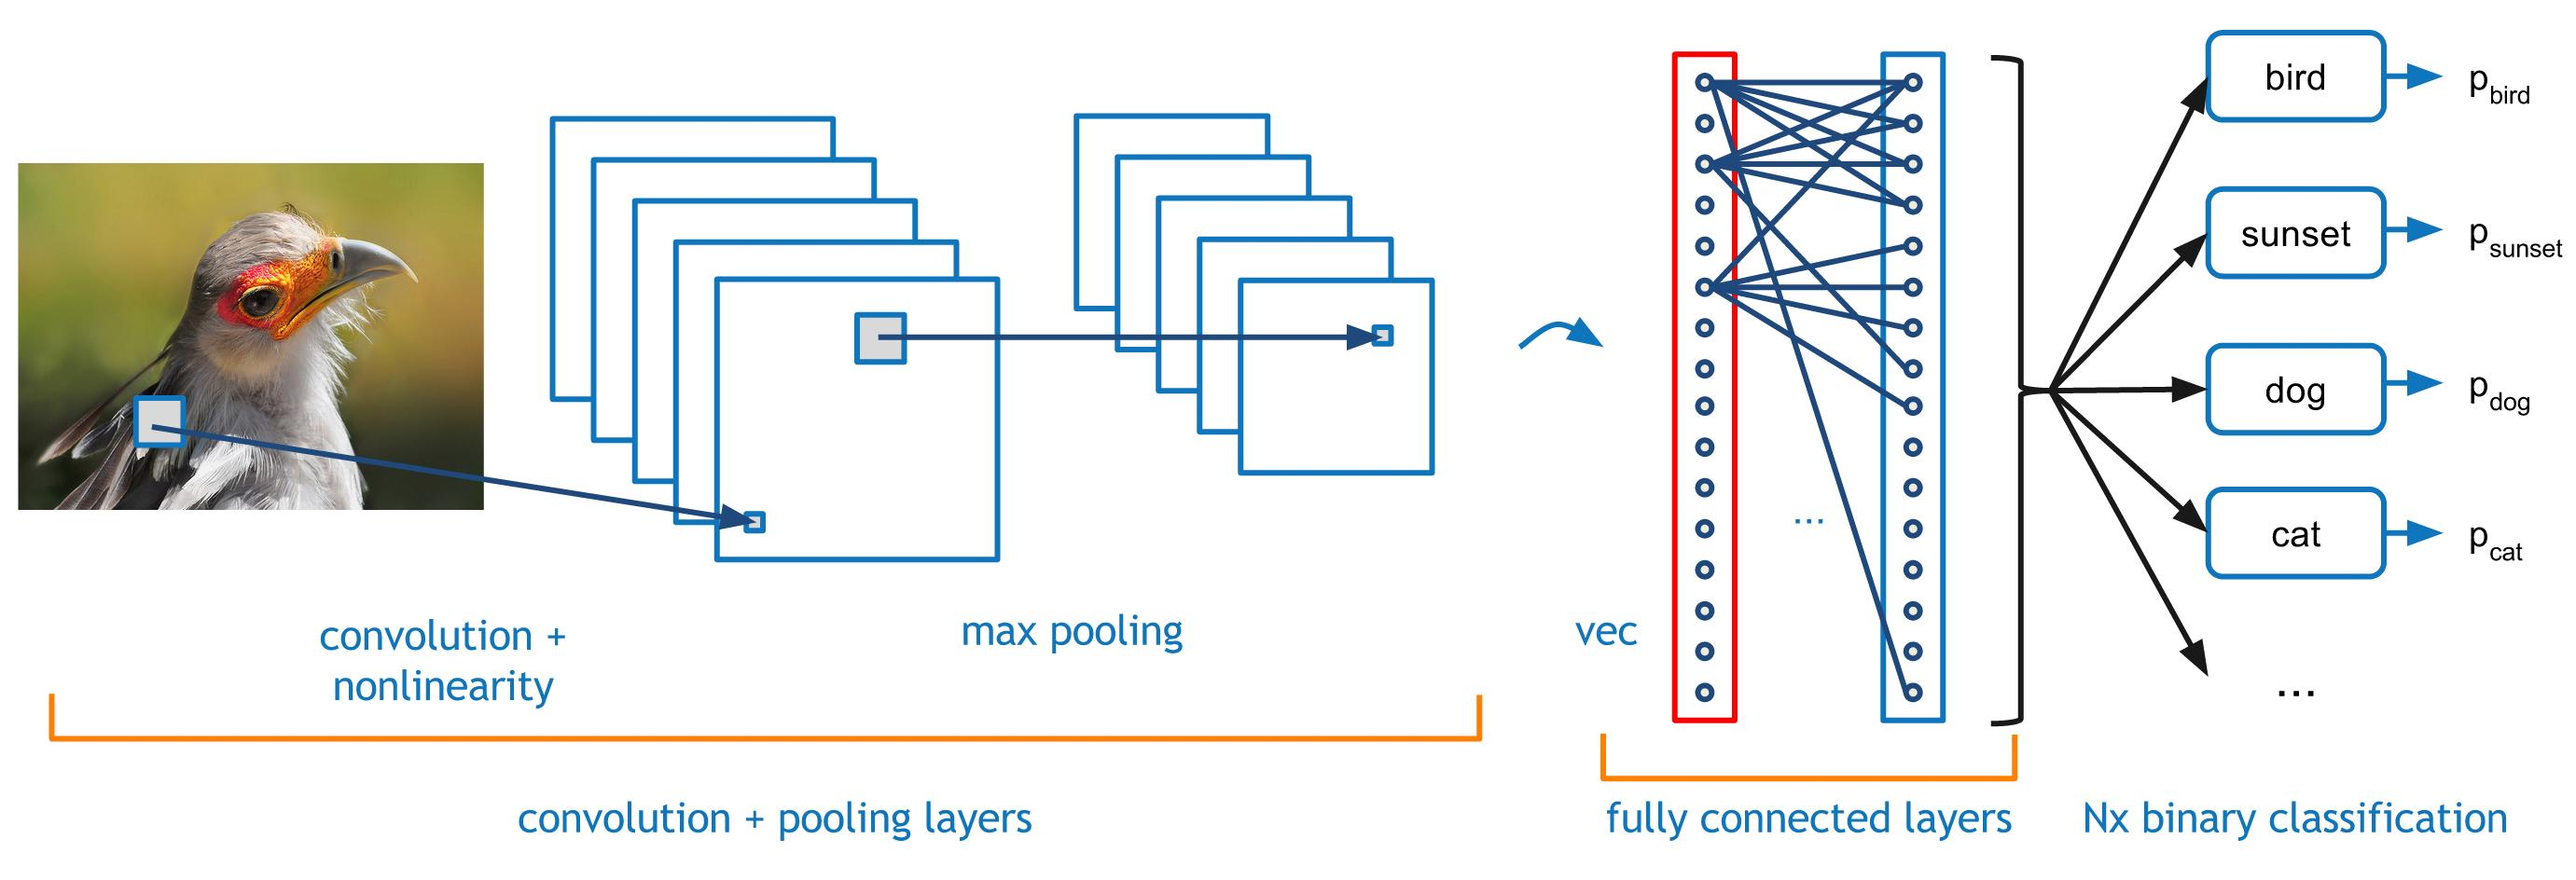
\includegraphics[width=1\textwidth]{../report/thesis_figures/conv-net2.jpg}
        \end{center}
    \end{figure}

    % show by hand neuron/layer
    % why conv works in images (less noise, pooling)
    % : add CNN figure
    % maybe add adversarial image
    % define ``features'' = last layer output
\end{frame}

\section{Visualization with t-SNE}
\begin{frame}
    \frametitle{Dimensionality Reduction with t-SNE}
    \begin{itemize}
        \item Definition of t-SNE % fixme: give acronym
        \item Optimized properties (spring model)
        \item Previous works
    \end{itemize}

    % : state-of-the-art for dim reduc, why we use it
    % already applied on mnist
\end{frame}

\begin{frame}
    \frametitle{Visualization with t-SNE}
    \begin{figure}[h]
        \begin{center}
            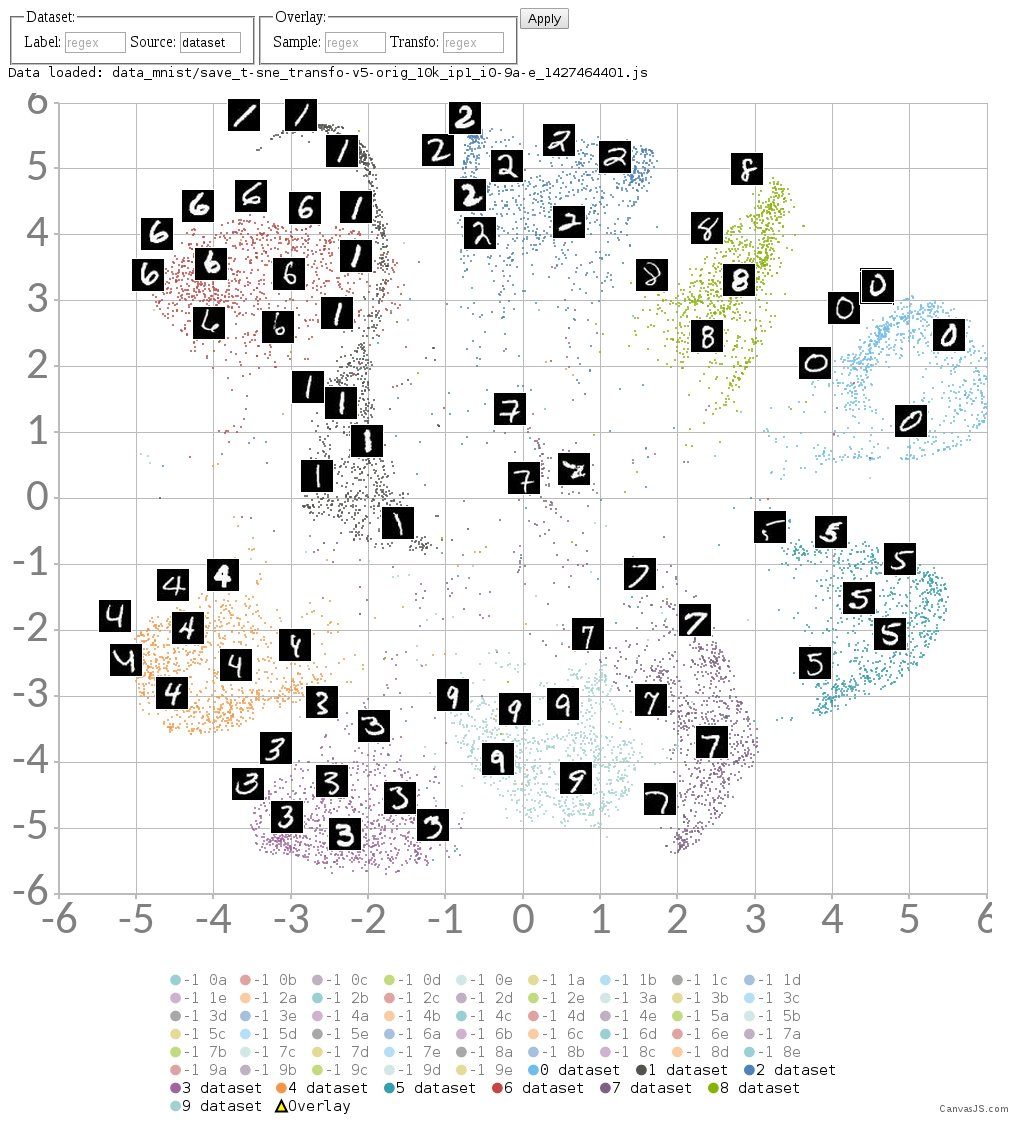
\includegraphics[width=0.8\textwidth]{../report/thesis_figures/mnist_nda_tsne.jpg}
        \end{center}
    \end{figure}
\end{frame}

\begin{frame}
    \frametitle{Visualization with t-SNE}
    \begin{figure}[h]
        \begin{center}
            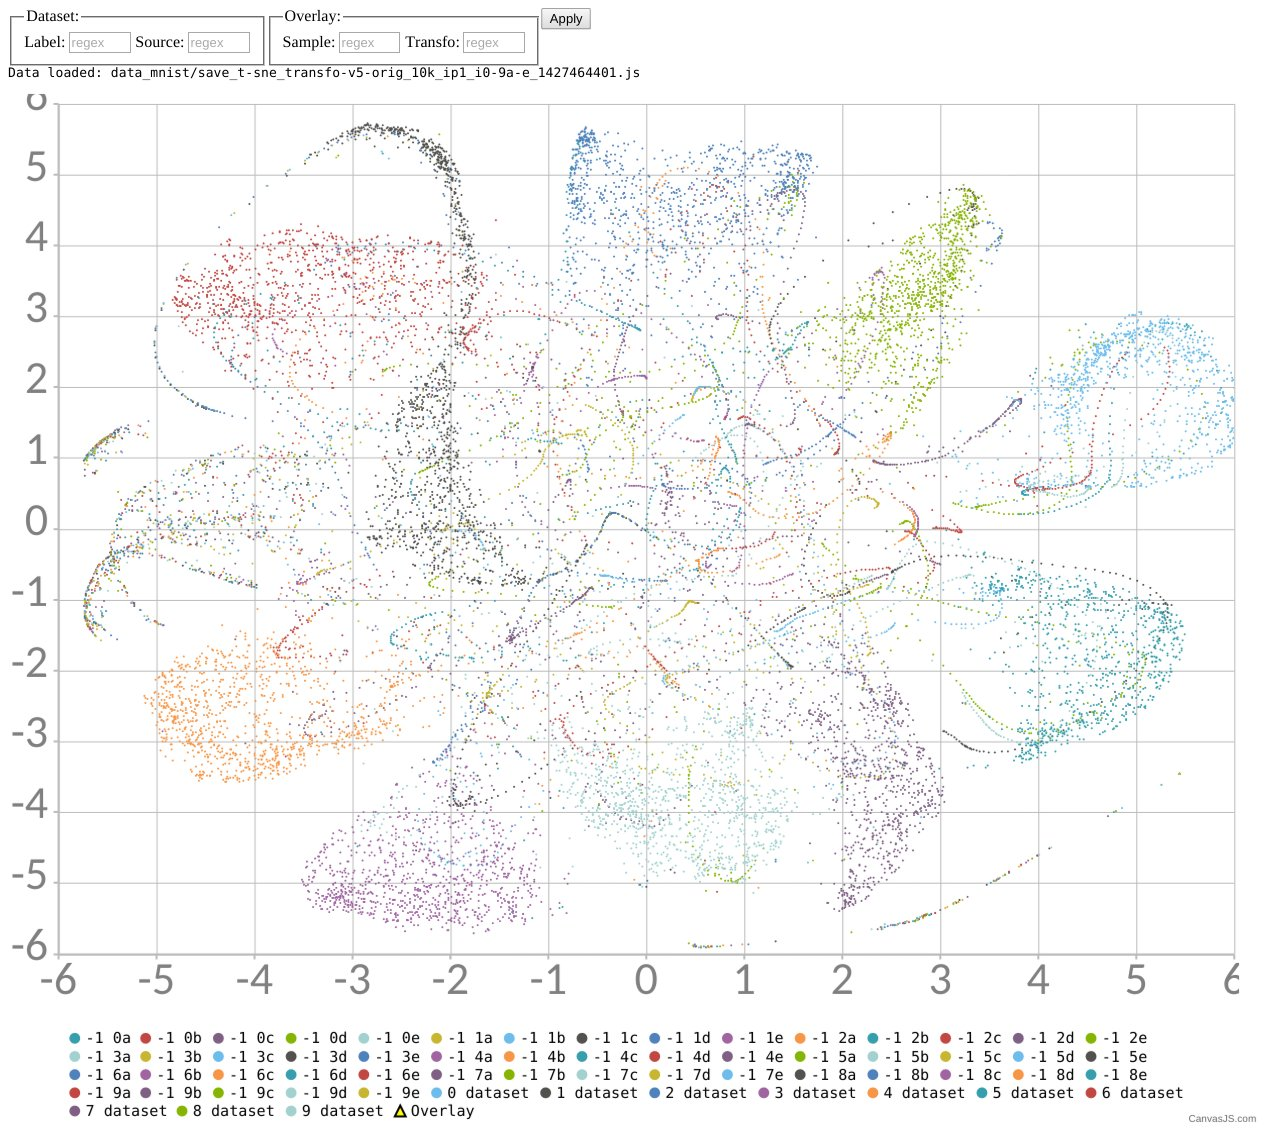
\includegraphics[width=0.5\textwidth]{../report/thesis_figures/mnist_nda_tsne2.jpg}
        \end{center}
    \end{figure}
    \begin{itemize}
        \item Results are unpredictable
        \item We could adapt t-SNE
    \end{itemize}
    However there exist better alternatives.

    % explain mnist
    % not really consistent

\end{frame}

\section{Towards Predictable Embeddings}
\begin{frame}
    % explain concepts
    \frametitle{Dimensionality Reduction with NN}
    \begin{itemize}
        \item DrLIM (Dimensionality Reduction by Learning an Invariant Mapping)
        \item Learn to reduce dimensionality directly using NN/CNN
    \end{itemize}

    \begin{figure}[h]
        \begin{center}
            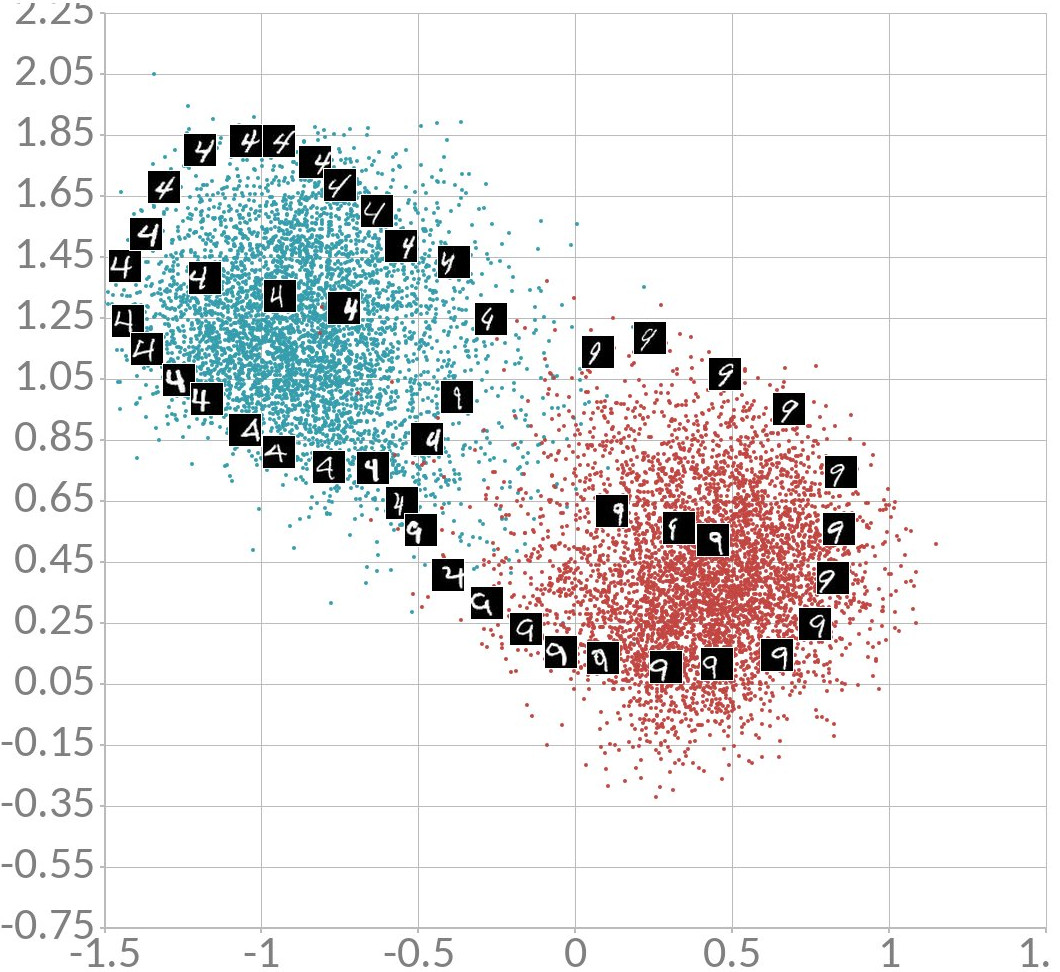
\includegraphics[width=0.65\textwidth]{../report/thesis_figures/mnist_cl_drlim.jpg}
        \end{center}
    \end{figure}
    %many pairing relations can be learned directly into embeddings.
    % explicit: it's DrLIM, not t-SNE, it's NN mapping, no projection, detail properties of this plot
\end{frame}

\begin{frame}
    \frametitle{Dimensionality Reduction with NN}
    Use:
    \begin{itemize}
        \item Siamese architecture % << figure
    \end{itemize}

    \begin{figure}[h]
        \begin{center}
            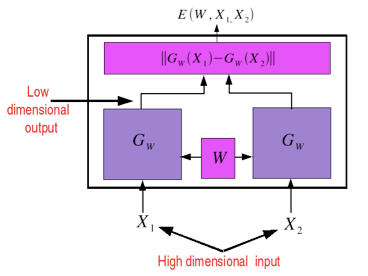
\includegraphics[width=0.75\textwidth]{../report/thesis_figures/siamese_network.jpg}
        \end{center}
    \end{figure}
\end{frame}

\begin{frame}
    \frametitle{Dimensionality Reduction with NN}
    And
    \begin{itemize}
        \item Contrastive loss
            \begin{eqnarray}
                L = \frac{1}{2} Y (D_W)^2 + \frac{1}{2} (1-Y) \max(0, m - D_W)^2
            \end{eqnarray}
    \end{itemize}
\end{frame}

\begin{frame}
    \frametitle{Predictable Embeddings}
    % first why we extend (we want predictable), why would it work (because more control, constraint component/dimensions correspond to relation)
    In our work we present:
    \begin{itemize}
        \item An extension of this loss for $N$ relations
            % change color the sum
            \begin{eqnarray}
                L = \frac{1}{2} \sum_{i=1}^p \left( Y_i (D_{Wi})^2 + (1-Y_i) \max(0, m_i - D_{Wi})^2 \right)
            \end{eqnarray}
        \item Qualitative and quantitative results
    \end{itemize}
\end{frame}

\begin{frame}
    \frametitle{Results On MNIST}
    \begin{itemize}
        \item Multiple parities at once
    \end{itemize}

    % this is same space, two projections
    % left one looks the same but we add the right

    \begin{figure}[h]
        \begin{center}
            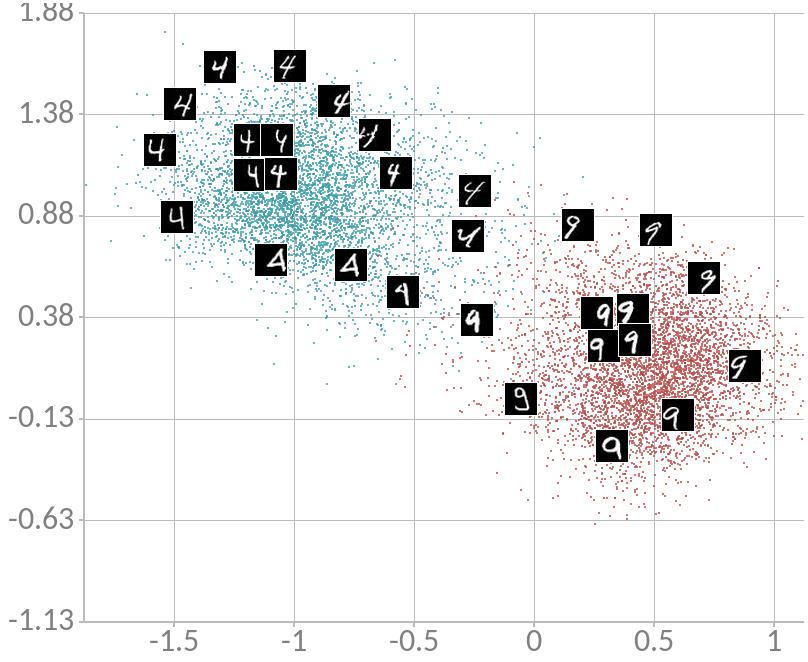
\includegraphics[width=0.45\textwidth]{figures/our_mnist.jpg}
            \vspace{1cm}
            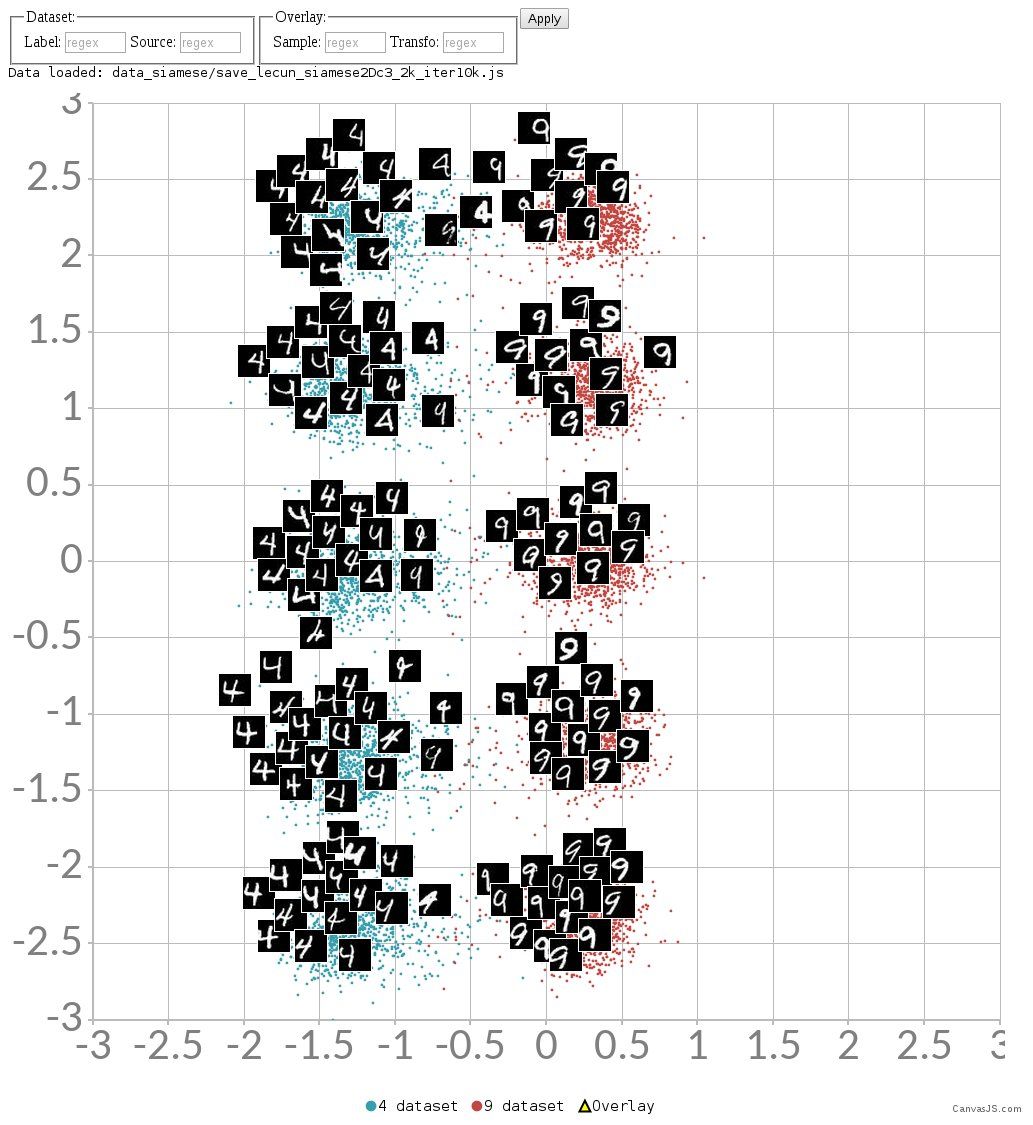
\includegraphics[width=0.5\textwidth]{../report/thesis_figures/mnist_cl2d2.jpg}
        \end{center}
    \end{figure}
\end{frame}

\begin{frame}
    \frametitle{Results On MNIST}
    \begin{itemize}
        \item Common loss function
    \end{itemize}

    \begin{figure}[h]
        \begin{center}
            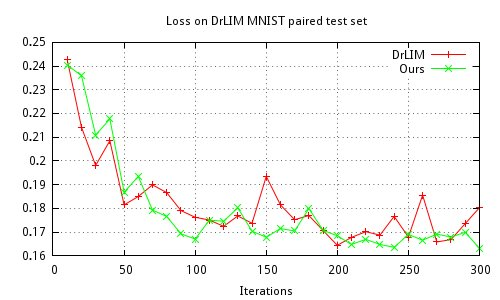
\includegraphics[width=0.8\textwidth]{../report/thesis_figures/final_loss_test2bv7.jpg}
        \end{center}
    \end{figure}
\end{frame}

% add slide for common loss

\begin{frame}
    \frametitle{Results On NORB}
    \begin{itemize}
        \item Comparison with DrLIM
    \end{itemize}


    % separate this slice: * show ours two viewpoints * briefly compare DrLIM and our (same viewpoint)
    \begin{figure}[h]
        \begin{center}
            \includegraphics[width=0.45\textwidth]{figures/drlim_norb.png}
            % zoom shape inside figure
            \vspace{1cm}
            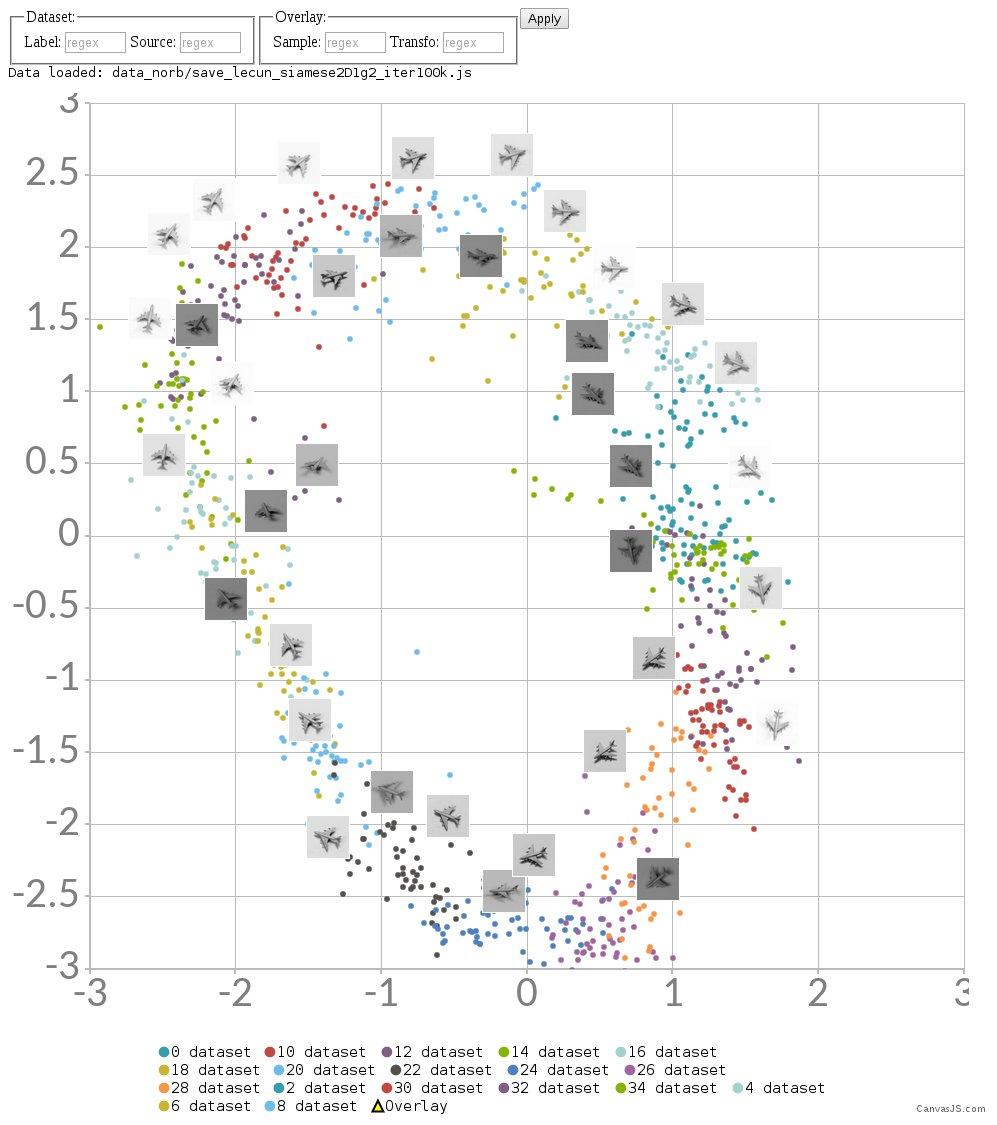
\includegraphics[width=0.45\textwidth]{../report/thesis_figures/norb_cl2d.jpg}
            % FIXME: add captions
        \end{center}
        \caption{left: DrLIM, right: our solution}
    \end{figure}
\end{frame}

\begin{frame}
    \frametitle{Results On NORB}
    \begin{itemize}
        \item Common loss function
    \end{itemize}

    \begin{figure}[h]
        \begin{center}
            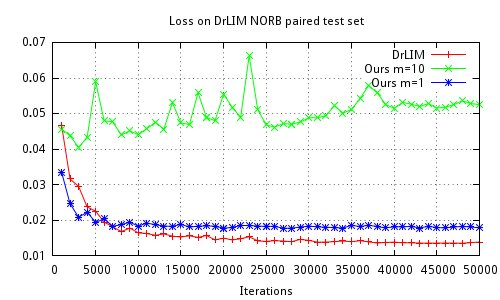
\includegraphics[width=0.8\textwidth]{../report/thesis_figures/final_loss_testv3.jpg}
        \end{center}
    \end{figure}
\end{frame}

\begin{frame}
    \frametitle{Results On NORB}
    \begin{itemize}
        \item More predictable structures
    \end{itemize}

    \begin{figure}[h]
        \begin{center}
            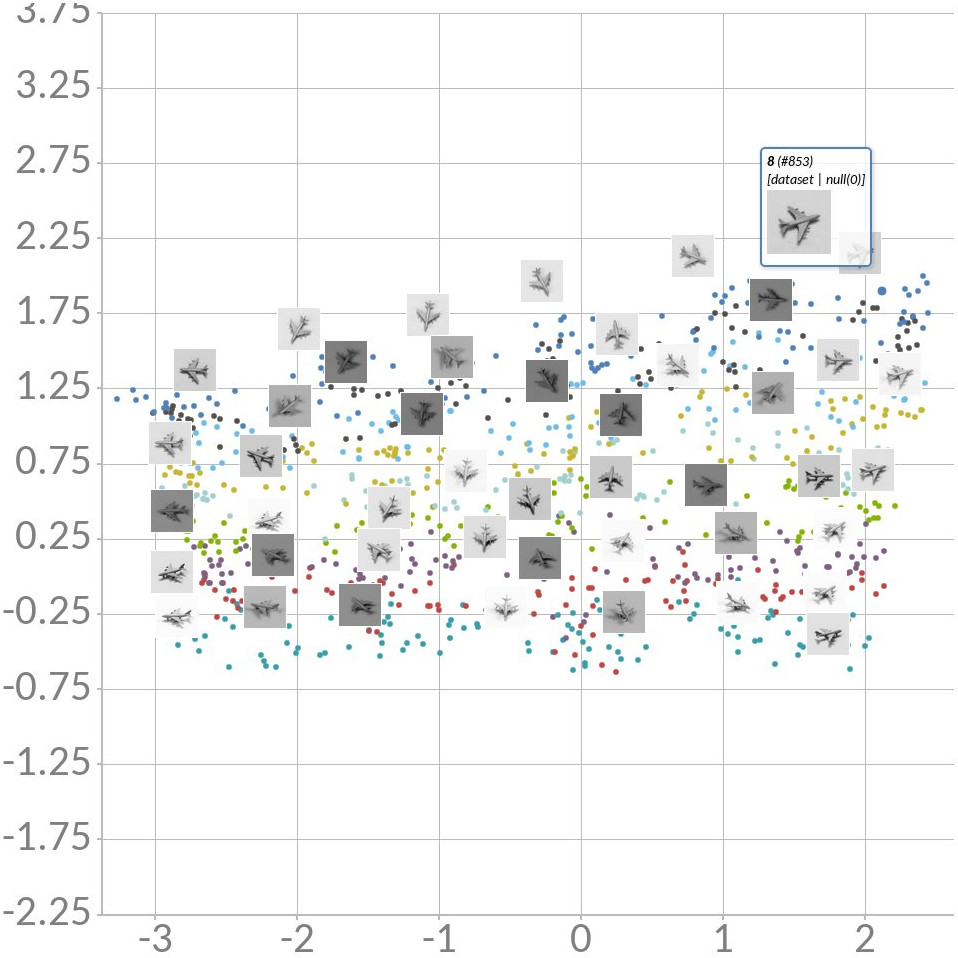
\includegraphics[width=0.45\textwidth]{../report/thesis_figures/norb_cl2d2.jpg}
            \vspace{1cm}
            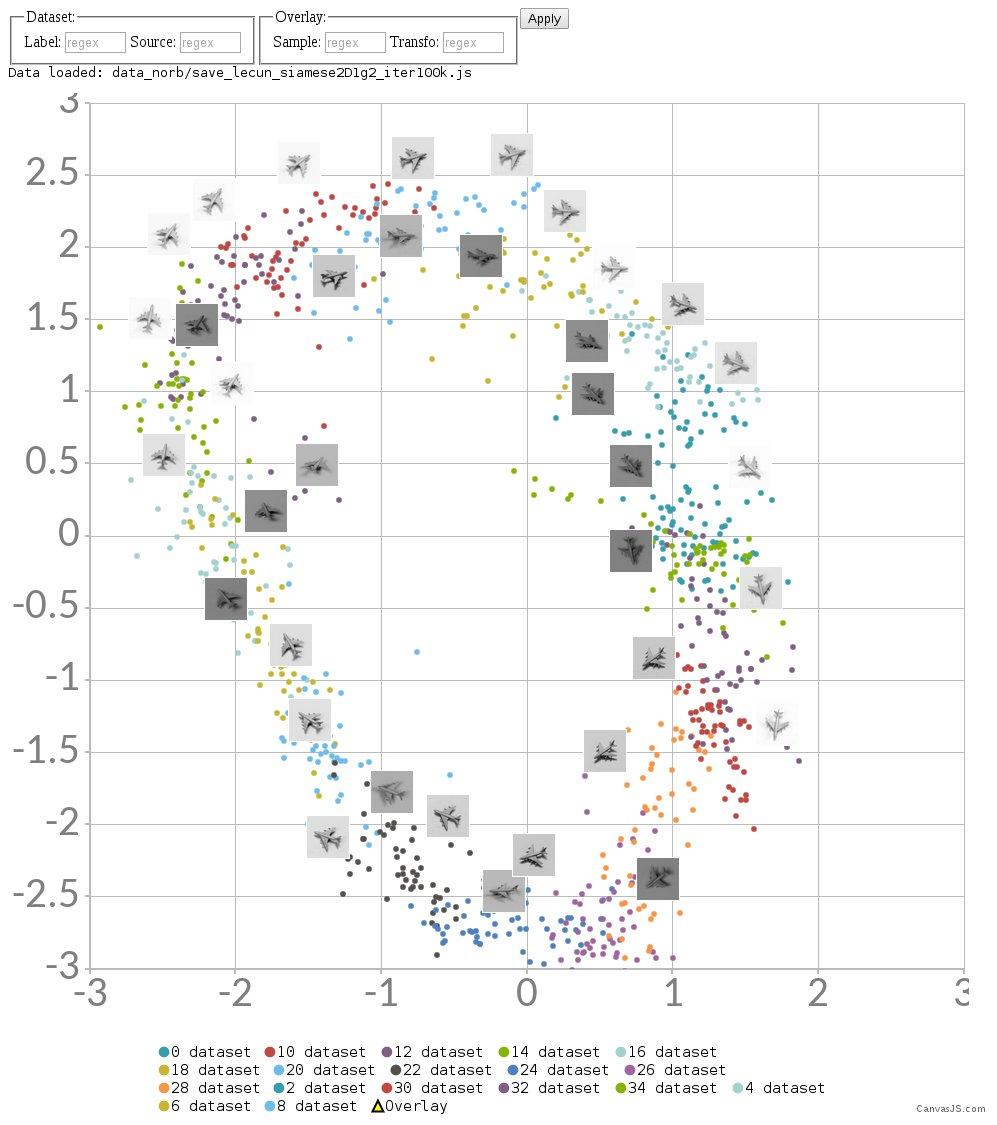
\includegraphics[width=0.45\textwidth]{../report/thesis_figures/norb_cl2d.jpg}
        \end{center}
    \end{figure}
\end{frame}

% add slide for common loss (we proposed quantitaive measures)
% what we choose, why (was not done before)

\section{Conclusion}
\begin{frame}
    \frametitle{Future Work}
    \begin{itemize}
        \item Make experimental comparisons with regression
        \item Show predictability with auxiliary networks
        \item Fields applications: Face Recognition, Bio-Medical Imaging.
    \end{itemize}
\end{frame}

% like summary
\begin{frame}
    \frametitle{Conclusion}
    \begin{itemize}
        \item Motivations of our work
        \item Unexpected results using t-SNE
        \item Proposition of an alternative with NN
        \item Further directions are promising
    \end{itemize}
\end{frame}

\begin{frame}
    \frametitle{Thank you}
\end{frame}

% appendix slides: t-sne formula
% fixme: more appendix slides?

\begin{frame}
    \frametitle{Appendix: t-SNE formula}
    \begin{eqnarray}
        L = \sum_{i=1}^n KL(P_i || Q_i) = \sum_{i=1}^n \sum_{j=1}^n p_{j|i} \log\left(\frac{p_{j|i}}{q_{j|i}}\right)
    \end{eqnarray}
    \begin{eqnarray}
        p_{j|i} = \frac{\exp(-|x_i - x_j|^2 / 2 \sigma_i^2)}{\sum_{k \not = i} \exp(-|x_i - x_k|^2 / 2 \sigma_i^2 )}
        %&
        %q_{j|i} = \frac{\exp(-|y_i - y_j|^2)}{\sum_{k \not = i} \exp(-|y_i - y_k|^2)}
        \end{eqnarray}
\end{frame}

\begin{frame}
    \frametitle{Appendix: Adversarial}
    \begin{figure}[h]
        \begin{center}
            \includegraphics[width=0.5\textwidth]{figures/adversarial1.png}
        \end{center}
    \end{figure}
\end{frame}

\end{document}
